\documentclass{article} % For LaTeX2e
\usepackage{cos424,times}
\usepackage{hyperref}
\usepackage{url}
\usepackage{graphicx}
\usepackage{amsmath}
%\usepackage{natbib}
\usepackage{multirow}
\usepackage{bm,bbm}
\usepackage{amssymb}
\usepackage{float}
\usepackage{subcaption}
\title{Fragile Families Challenge}

\author{
Andrew Or\\
Department of Computer Science\\
Princeton University\\
\texttt{andrewor@cs.princeton.edu} \\
\And
Thomas Shaffner \\
Department of Computer Science \\
Princeton University \\
\texttt{tfs3@cs.princeton.edu} \\
}

\newcommand{\fix}{\marginpar{FIX}}
\newcommand{\new}{\marginpar{NEW}}

\begin{document}

\maketitle

\begin{abstract}

This paper describes our submission to the Fragile Families Challenge \cite{ffc}, an effort that applies techniques in predictive modeling and causal inference to interviews conducted with disadvantaged families. The goal of the project is to improve the lives of children in these families by identifying underlying patterns in the answers given by the families. In this work, we use regression and classification methods to predict the values of six key attributes: GPA, grit, material hardship, eviction, layoff, and job training. Because of the abundance of invalid entries in the data, feature selection plays a crucial role in our effort.

\end{abstract}
\section{Introduction}
\label{sec:intro}

The Fragile Families and Child Wellbeing Study (FFCWS) \cite{ffcws} is an academic collaboration that follows around 5,000 urban families in the United States and collects information about how their social environments change over time. Interviews were first conducted shortly after the birth of the family's child between 1998 and 2000, then were conducted again when the child was age one, three, five, nine, and fifteen. Because of the goal is to understand the difficulty face by disadvantaged families, non-marital births are overrepresented (roughly three-quarters of all births) in the study.

The data collected in this study has been used by academic papers published in many journals since then \cite{ffc_publications}. Insights derived from this data are shared with policy makers through the Future of Children \cite{foc}, a collaboration between the Woodrow Wilson School of Public and International Affairs at Princeton University and the Brookings Institution.

The Fragile Families Challenge is an open challenge for data scientists to apply machine learning and statistical methods to the data collected in this study. The challenge aims to use ensemble methods on the best models submitted to discover factors correlated with children beating the odds.

In this paper, we propose our solution to the Fragile Families Challenge. We modeled continuous labels and binary labels separately, using regression methods for the former and classification methods for the latter. The regression methods we evaluated are:

\begin{enumerate}
\item Linear Regression with Lasso Regularization
\item Support Vector Regression
\item Random Forest Regression
\end{enumerate}
and the classifiers we evaluated are:
\begin{enumerate}
\item Bernoulli Naive Bayes Classifier
\item Multinomial Naive Bayes Classifier
\item K-Nearest Neighbors Classifier
\item Random Forest Classifier
\item Gradient Boosting Classifier
\end{enumerate}

We used the \texttt{sklearn} implementation of all of the above regression and classification methods. The main metrics we used in our evaluation are the coefficient of determination (also known as the $R^2$ score) for continuous labels and accuracy for binary labels. In both cases, we found that Random Forest performs the best. To account for the abundance of missing or invalid values in the dataset, we experimented with various feature selection and imputation techniques, as we discuss next.

All source code is available on Github at \cite{myrepo}.

\section{Dataset}
\label{sec:dataset}

The background data is primarily composed of answers collected from interviews with the families over the years. These are the features used to train our models. Each row uniquely identifies a child and each column is either an ID of some form or an interview answer. In this dataset, there are 4242 rows and 12945 columns.

The label data consists of six labels we wish to predict based on the features in the background data. There are 2121 rows in the label data, exactly half the number of rows in the background data. The goal is to predict the six labels for the 2121 missing rows. These labels are derived from a final interview with the child when he or she is age 15. The six labels are: GPA, grit, material hardship, eviction, layoff and job training. The first three are continuous labels while the latter three are binary labels.

% We used two datasets in this experiment. The first is the Sentiment Labelled Sentences Data Set \cite{smalldataset}, which consists of 3,000 labelled sentences extracted from reviews from IMDB, Amazon, and Yelp. There are 500 positive and 500 negative sentences from each of the websites and no neutral sentences. This dataset was used for evaluating a classification method that works around the lack of instance labels by exploring instance-level similarity \cite{individuallabel}.

% The second dataset used in this experiment is the Multi-Domain Sentient Dataset \cite{largedataset}, which contains 38548 Amazon biased reviews. The subset used in this project is comprised of 10,000 reviews randomly sampled from all product categories. Prior work has used this dataset for a variety of purpose, ranging from sentiment classification \cite{domainadaptation} to providing bounds for minimizing empirical risk \cite{learningbounds} to weighting linear classifiers with confidence \cite{confidenceweight}.

% The reasons for using this second dataset are twofold. First, it is much larger than the first one, which is conducive to more general models and thus lower generalization error. Many commonly used text analysis techniques we explored did not have a significant impact on the accuracy when training on the smaller dataset. Second, the Amazon dataset comes with ratings (out of 5 stars) in addition to just positive or negative labels. This enables us to generalize the techniques used in this project to multi-class classification in the future.

\section{Preprocessing}
\label{sec:preprocessing}

[TODO: WRITE ME]

% Raw word tokens are not suitable as features for several reasons. First, some words are used only very rarely and do not actually convey any sentiment. These could be words that are highly specific to the user or simply typos. Second, many words have multiple forms that are semantically equivalent. Third, analyzing individual word tokens misses semantics expressed through phrases or negation. Thus, feature extraction and selection are both conducive to a feature set more representative of the underlying sentiments expressed by the users.

\subsection{Imputation}
\label{sec:imputation}

[TODO: WRITE ME]

\subsection{Feature selection}
\label{sec:featureselection}

[TODO: WRITE ME]

% Without any feature selection, the number of features extracted this way is 11252 for the smaller dataset and 166566 for the larger dataset. Especially in the latter case, classifying on this many features is prohibitively expensive and prone to noise.

% Thus, we filtered the number of features as follows. First, we removed stop words, as specified by the NLTK library, and any words that occurred fewer than 5 times in the corpus. This step alone reduced the number of features to 515 in the smaller dataset and 6666 in the larger dataset. Then, we ranked the remaining features by Chi-squared score, which is given by:

% \begin{align*}
% \chi^2 = \sum_{ij}{\dfrac{(O_{ij} - E_{ij})^2}{E_{ij}}}
% \end{align*}

% where $O_{ij}$ is the observed count and $E_{ij}$ is the expected count. This quantity measures how much observed counts deviate from expected counts and tests the independence between two variables: the feature variable and the class variable in our case. We then select the best $k$ (lowest $\chi^2$) features and use them for classification.

% We experimented with different values of $k$ depending on the dataset. For the smaller dataset, we used $k = 463$, which throws approximately 10\% of the remaining features after removing rare words and stop words. For the larger dataset, we used $k = 4000$, which throws about around 40\% of the remaining features.

\section{Regression}
\label{sec:regression}

We tested several classification and regression methods (detailed in Section~\ref{sec:intro}), but ultimately used random forest methods for both classification and regression tasks. Here we discuss in more detail the specifics of random forest regression.

Random forest regression methods are used to combine multiple regression trees. The random forest regression algorithm draws uniformly at random $m$ subsets of the training data. The algorithm then trains a regression tree on each of the subsets.

\begin{figure}[H]
  \centering
  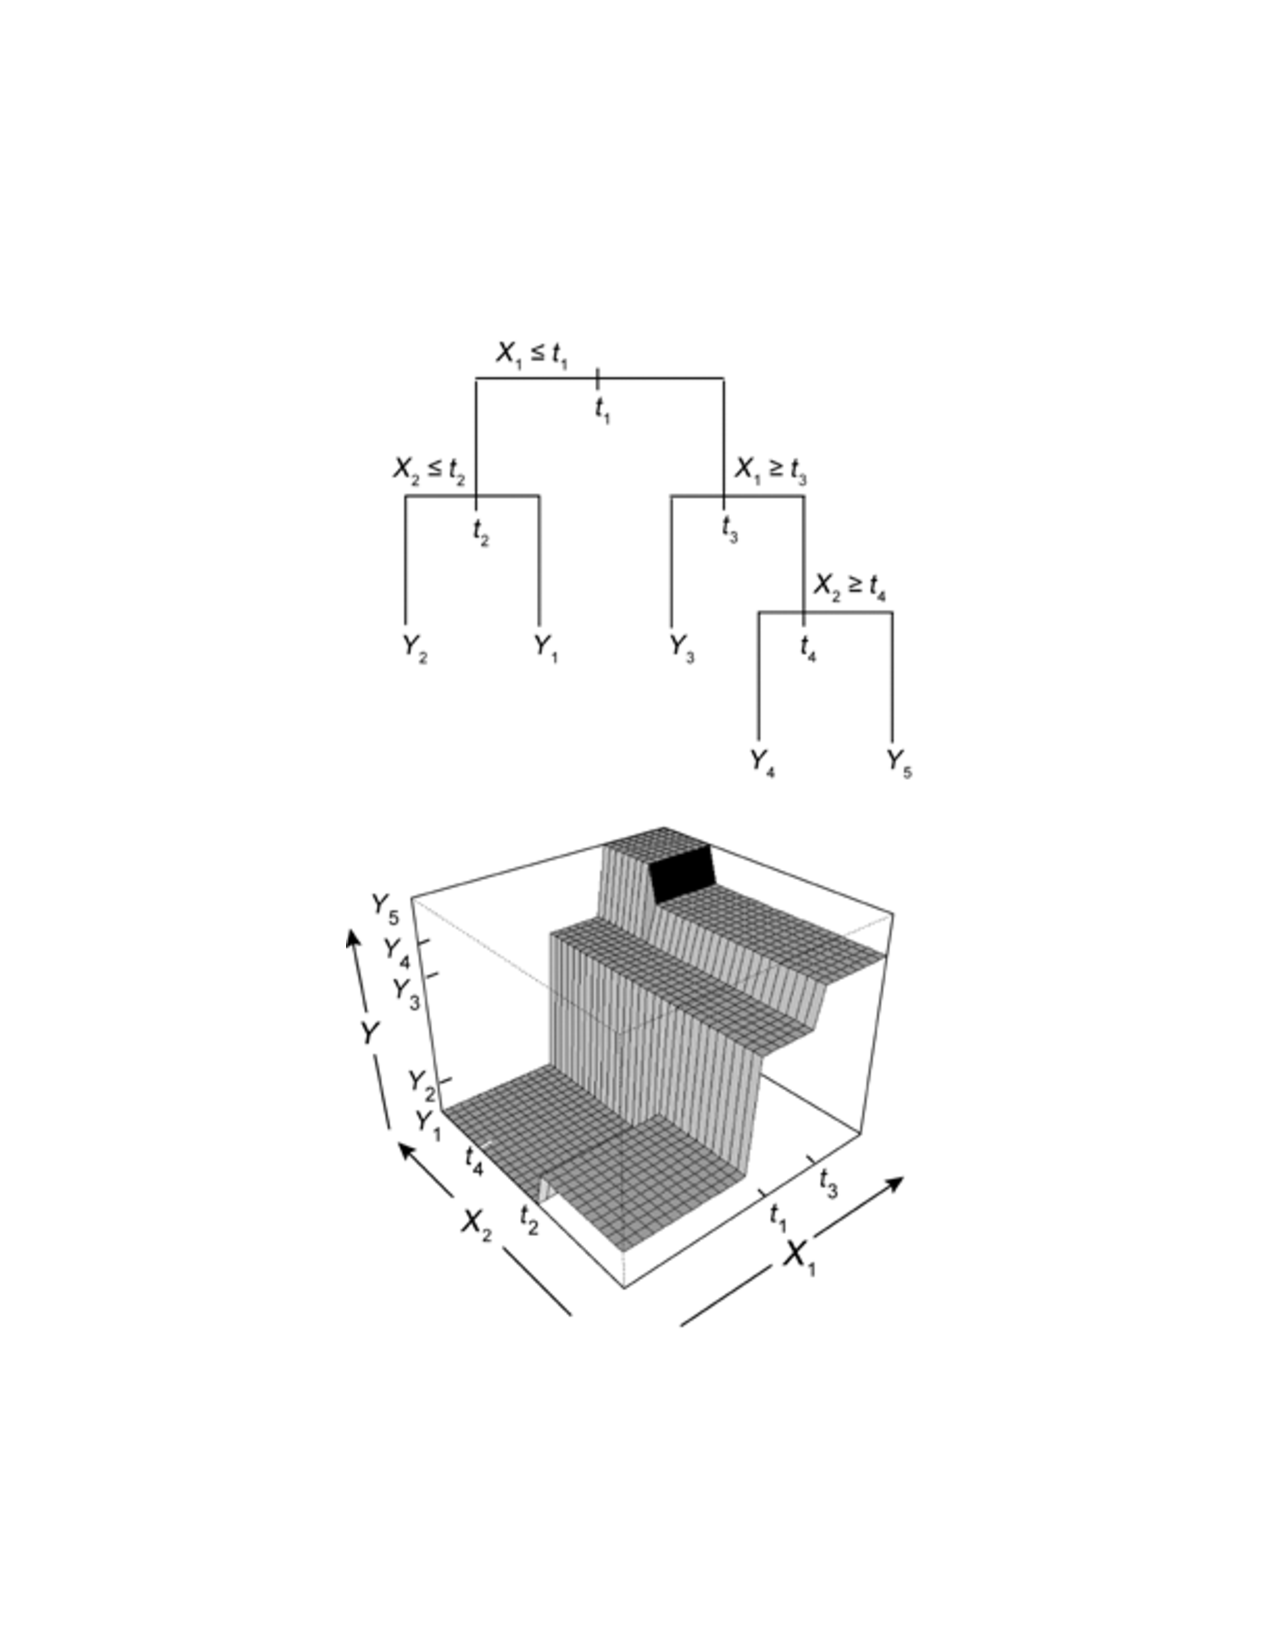
\includegraphics[trim={0 6cm 0 6cm}, width=0.75\textwidth]{rt.pdf}
  \caption{An example regression tree, borrowed from \cite{rffig}}
  \label{fig:regtree}
\end{figure}

In the same manner as decision trees, regression trees split samples at branch points based on feature values (see Figure~\ref{fig:regtree}). Given training samples $x_i$ and (continuous) training response variables $y_i$, regression trees are built in the following manner.

\begin{enumerate}
  \item Select the optimal feature $f$ and value $v_f$ for branching by minimizing $RSS$
  \item Partition samples into $L = \{i | x_{if} \leq v_f\}$ and $R = \{j | x_{jf} > v_f\}$
  \item Recurse on the subsets $L$ and $R$ of input data
\end{enumerate}

with $RSS$ defined as

\begin{align*}
  RSS &= \sum_{i \in L} (y_i - y_L^*)^2 + \sum_{j \in R} (y_j - y_R^*)^2
\end{align*}

and where $y_L^* = \frac{1}{\lvert L \rvert} \sum_{i \in L} y_i $ is the mean of all response variables corresponding to samples in the left subtree of the branch point, and $y_R^* = \frac{1}{\lvert R \rvert} \sum_{j \in R} y_j$ is the mean of all response variables corresponding to samples in the righthand subtree.

Given a new sample $x$, a single regression tree determines which leaf represents $x$ and assigns to $x$ the predicted $y$ value of the mean of all response values represented by that leaf. Random forest regressors, given a new sample $x$, return as a prediction the average of the responses of each regression tree.

% We trained four different models using this set of features: Bernoulli naive Bayes, multionmial naive Bayes, decision trees, and random forests. In this section, we will discuss random forests in detail.

% Random forest \cite{randomforest} is an ensemble learning method used for classification and other machine learning tasks. The central idea behind random forest is bootstrap aggregating, also known as bagging, a technique that combines the results of multiple learning algorithms to reduce variance and avoid overfitting.

% The algorithm generates $B$ random subsets of the input data and trains a decision tree on each one of the subsets. Additionally, in the spirit of the random subspace method \cite{randomsubspace}, each decision tree chooses $d$ features sampled randomly with replacement from the original set of features. Then, to predict a data point, the algorithm traverses all $B$ decision trees and returns the mode as the predicted label.

% \begin{figure}[H]
%   \centering
%   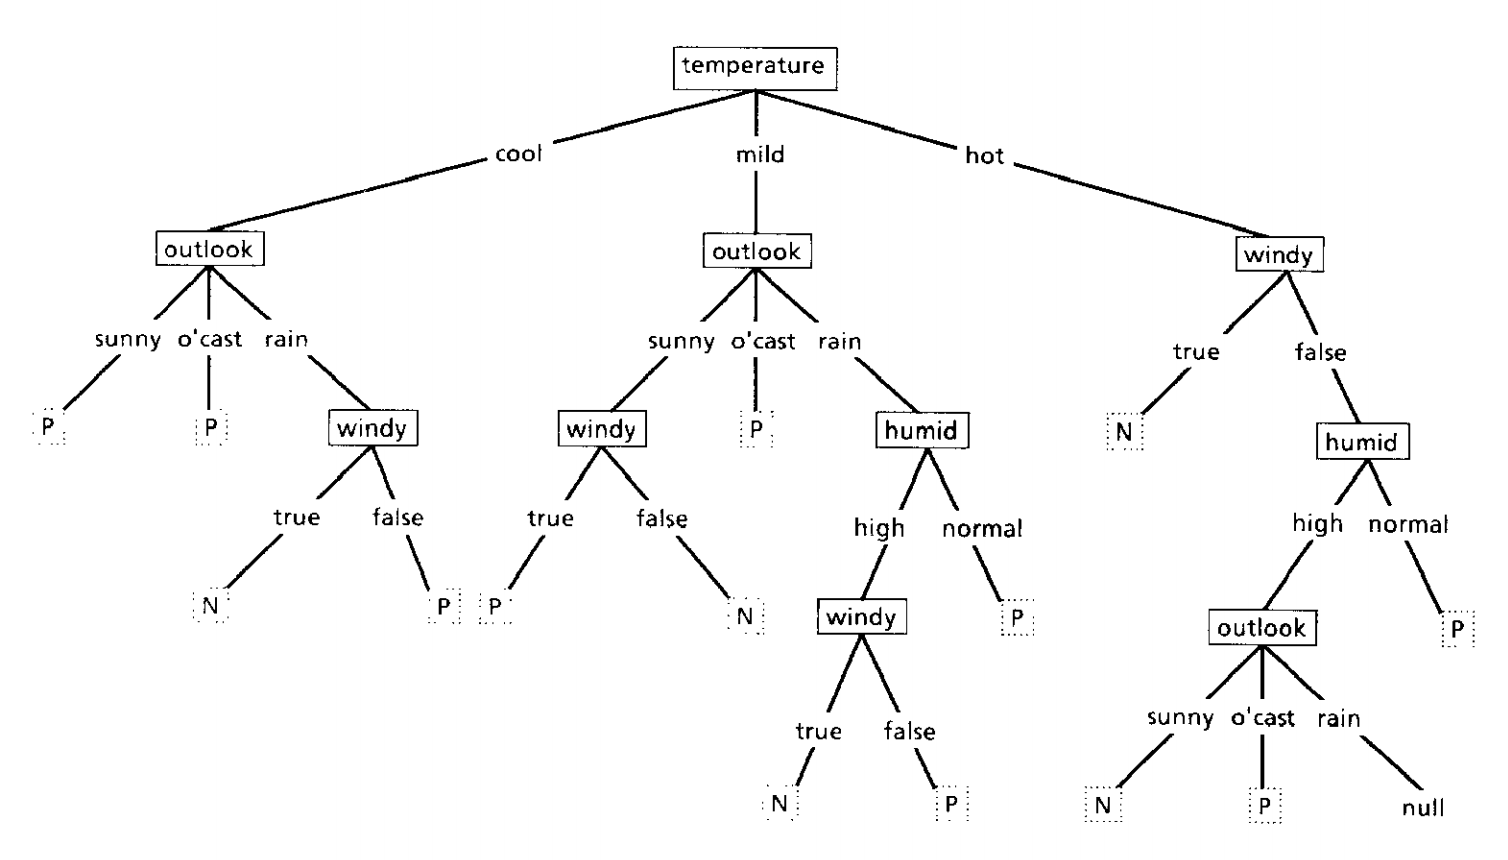
\includegraphics[width=0.9\textwidth]{dt.png}
%   \caption{A complex decision tree, borrowed from \cite{id3}}
% \end{figure}

% Each decision tree can be built as follows using the ID3 algorithm \cite{id3}:
% \begin{enumerate}
% \item Select the best feature that minimizes entropy (or maximizes information gain)
% \item Split input data by the values of the feature, creating a node for each value
% \item Recurse on each node by selecting the best remaining features
% \end{enumerate}

% Entropy is defined as follows:
% \begin{align*}
% \mathbb{H}(\pi) = -\sum_{c=1}^{C}{\pi_c log(\pi_c)}\\
% \pi_c = \dfrac{1}{|\mathcal{D}|}\sum_{i \in \mathcal{D}}{\mathbb{I}(y_i = c)}
% \end{align*}
% where $\mathcal{D}$ is the data in the leaf node. Then information gain between the parent node $Y$ and the child node representing the test $X_j < t$ is given by \cite{textbook}:
% \begin{align*}
% IG(X_j < t, Y) &= \mathbb{H}(Y) - \mathbb{H}(Y | X_j < t)\\
% &=\left(-\sum_c{p(y=c) \log p(y=c)}\right) + \left(\sum_c{p(y=c|X_j < t)\log p(c|X_j < t)}\right)
% \end{align*}

% The motivation behind combining the results of many decision trees is that single decision trees are highly sensitive to noise in the training set and thus prone to overfitting. Combining multiple decision trees reduces the variance of the model as long as the individual trees are not correlated. This requirement is provided by building trees on different subsets of the input data and using different a subset of features on each tree.

\section{Evaluation}
\label{sec:evaluation}

[TODO: WRITE ME]

% We used implementations in the \texttt{scikit-learn} \cite{scikitlearn} library for each of the classification schemes described above. Additionally, as a thought experiment, we implemented our own Bernoulli naive Bayes and multinomial naive Bayes classifiers from scratch in python and compared our results against implementations in \texttt{scikit-learn}. To enhance the robustness and generality of each of our models, we used $k$-fold cross validation with $k=5$.

\subsection{Metrics}
\label{sec:metrics}

[TODO: WRITE ME]

% In addition to raw accuracy, we evaluated each of the classification methods using a number of standard classification metrics.
% \begin{align*}
% &\text{Area under ROC curve}\\
% \text{precision} &= \dfrac{TP}{TP + FP}\\
% \text{recall} &= \dfrac{TP}{TP + FN}\\
% \text{F1 score} &= 2 \cdot \dfrac{\text{precision} \cdot \text{recall}}{\text{precision} + \text{recall}}
% \end{align*}

% These additional metrics were chosen because the raw accuracy does not contain any information about the number of false positives and false negatives. The area under the ROC curve gives us insight into the probability that a randomly chosen positive example has higher probability in being predicted as positive than a randomly chosen negative example. However, the area under two ROC curves can still be equal even if the two models have widely different precision and recall. Since precision and recall are both desirable properties, we use the F1 score, which captures the harmonic mean of both rates, in our evaluation.

\subsection{Hyperparameter tuning}
\label{sec:hyperparametertuning}

[TODO: WRITE ME MORE]

For continuous variables, we used the $\texttt{GridSearchCV}$ method from the $\texttt{scikit-learn}$ Python package to tune hyperparameters using cross-validation. We examined all combinations of hyperparameters in Figure~\ref{fig:contparams}. $\texttt{n\textunderscore estimators}$ represents the number of regression trees trained, $\texttt{max\textunderscore features}$ represents the portion of all features to examine while generating splits, and $\texttt{min\textunderscore samples\textunderscore split}$ represents the minimum number of samples in a node before it is allowed to split.

\begin{figure}[H]
  \centering
  \begin{subfigure}[b]{0.35\textwidth}
    \begin{align*}
      &\texttt{[TODO: WRITE~ME]}
    \end{align*}
    \caption{Options for boolean classification}
    \label{fig:boolparams}
  \end{subfigure}
  \hfill
  \begin{subfigure}[b]{0.35\textwidth}
    \begin{align*}
      &\texttt{n\textunderscore estimators}:~50,~75,~100\\
      &\texttt{max\textunderscore features}:~0.75,~1.0\\
      &\texttt{min\textunderscore samples\textunderscore split}:~10,~25,~50
    \end{align*}
    \caption{Options for continuous regression}
    \label{fig:contparams}
  \end{subfigure}
  \caption{Hyperparameter options}
  \label{fig:params}
\end{figure}

% The default parameters of the decision tree and random forest classifiers in \texttt{scikit-learn} did not yield good accuracy. Thus, for these models, we experimented with different sets of hyperparameters by trial and error. More specifically, the parameter grid we explored was:
% \begin{align*}
% &\texttt{min\textunderscore leaf\textunderscore samples}: 1, 10, 100\\
% &\texttt{max\textunderscore features}: 0.5, 0.75, 0.9\\
% &\texttt{n\textunderscore estimators}: 10, 30, 100
% \end{align*}
% where last parameter is for random forest only. We chose to tune \texttt{min\textunderscore leaf\textunderscore samples} because the default was 1, which led to many splits that were overly specific to the training set. Similarly, tuning \texttt{max\textunderscore features} reduces the chance of overfitting. Using more trees by increasing \texttt{n\textunderscore estimators} further randomizes the training, which should lead to lower generalization errors. In our experiments, we found that the best hyperparameters to use are $\texttt{min\textunderscore leaf\textunderscore samples} = 1, \texttt{max\textunderscore features} = 0.9, \texttt{n\textunderscore estimators} = 100$ for the smaller dataset and $\texttt{min\textunderscore leaf\textunderscore samples} = 10, \texttt{max\textunderscore features} = 0.9, \texttt{n\textunderscore estimators} = 100$ for the larger dataset.

\subsection{Results}
\label{sec:results}

[TODO: WRITE ME]

% \begin{table}[htbp]
% \small
%    \centering
%    \begin{tabular}{|c|c|c|c|c|c|c|c|c|c|c|}
%    \hline
%     &  \multicolumn{5}{c|}{2,400 sentiment labelled sentences} &
%   \multicolumn{5}{c|}{10,000 Amazon reviews}  \\
%   \cline{2-11}
%    Classifier & Acc & Prec & Recall & $F_1$ & AUC ROC & Acc & Prec & Recall & $F_1$ & AUC ROC \\ \hline \hline
%    mybnb & 0.71 & 0.67 & 0.76 & 0.71 & 0.69 & 0.51 & 0.68 & 0.27 & 0.38 & 0.55 \\\hline
%    mymnb & 0.69 & 0.66 & 0.75 & 0.69 & 0.68 & 0.66 & 0.75 & 0.61 & 0.67 & 0.67 \\\hline
%    bnb & 0.62 & 0.66 & 0.68 & 0.62 & 0.75 & 0.78 & 0.78 & 0.85 & 0.81 & 0.86 \\\hline
%    mnb & 0.62 & 0.65 & 0.69 & 0.63 & 0.75 & 0.79 & 0.81 & 0.83 & 0.82 & 0.86 \\\hline
%    dt & 0.62 & 0.62 & 0.70 & 0.63 & 0.65 & 0.70 & 0.72 & 0.78 & 0.75 & 0.75 \\\hline
%    rf & 0.60 & 0.65 & 0.56 & 0.57 & 0.69 & 0.73 & 0.74 & 0.82 & 0.78 & 0.81 \\\hline
%    \end{tabular}
%    \caption{Accuracy, precision, recall, F1 score, and area under ROC curve for all models evaluated under two datasets of different sizes using 5-fold cross validation. \texttt{mybnb} and \texttt{mymnb} refer to the custom implementation of Bernoulli naive Bayes and multinomial naive Bayes respectively. The rest of the classifiers use implementations provided by \texttt{scikit-learn}.}
%    \label{tab:classifiers}
% \end{table}

% Table~\ref{tab:classifiers} shows that the characteristics of each of the classification methods vary across datasets. Training the model on the larger dataset generally improves all metrics compared to training it on the smaller dataset. The notable exceptions are \texttt{mybnb} and \texttt{mymnb}, which are custom python implementations of Bernoulli naive Bayes and multinomial naive Bayes respectively. These simplistic implementations actually outperform their counterparts in \texttt{scikit-learn} for small datasets, but do not scale as well to larger datasets.

% Our experiments show that \texttt{bnb} and \texttt{mnb} yield the best results among all the classifiers we explored. Even on the smaller dataset, although all the classifiers have similar accuracy, \texttt{bnb} and \texttt{mnb} have consistently higher area under the ROC curve than \texttt{dt} and \texttt{rf}. When extended to the larger dataset, the difference becomes more pronounced, both in terms of the AUC and all other metrics.

% These results are somewhat surprising; despite tuning the hyperparameters, we still saw low accuracy on \texttt{rf} relative to the linear classifiers. The following is one potentially illuminating example taken from the Amazon dataset. The sentiment is negative (0) but the scores given by \texttt{dt} and \texttt{rf} are 0.86 and 0.81 respectively, while the scores given by \texttt{bnb} and \texttt{bnb} are 0.28 and 0.30 respectively.

% \begin{quote}
% This video's only redeeming quality is its excellent pilates instruction. Like all Stott videos this one takes extra care to explain proper form and technique. Unfortunately, the aerobics portion is extremely boring and simple. You just walk in place the whole time with no interesting variations.
% \end{quote}

% This example is potentially confusing because it contains many words that are strongly correlated with positive or negative sentiments, such as 'excellent', 'proper', 'unfortunately', 'boring'. However, neither the tree classification methods nor the naive Bayes methods were lukewarm about their answers (i.e. reporting a score around 0.50). The certainty that this example is positive (which is incorrect) is only reduced from 0.86 to 0.81 when switching from \texttt{dt} to \texttt{rf} with 100 trees, suggesting that the number of trees may still be too low or the hyperparameters may not be sufficiently tuned. It is also possible that even the larger dataset used in this experiment is not sufficiently large for random forests to generalize well.

\section{Conclusion}
\label{sec:conclusion}

[TODO: WRITE ME]

% We evaluated four different classification methods on two datasets of different sizes. We found that the multinomial naive Bayes classifier achieved highest accuracy, precision and recall. Based on similar studies, we suspect that the random forest classifier could achieve better results with more trees, more careful hyperparameter tuning, and larger datasets. It may also be worthwhile to investigate other measures of information gain, such as the gini impurity.

% Another future direction is to generalize this classification to multiple classes, one for each star (out of five). Preliminary work from this project demonstrated that it is much more difficult to achieve high accuracy in this task, however, since ratings are highly subjective to the user.

\begin{thebibliography}{}

\bibitem{myrepo}
https://github.com/andrewor14/ffc

\bibitem{ffc}
Fragile Families Challenge: http://www.fragilefamilieschallenge.org/

\bibitem{ffcws}
Fragile Families and Child Wellbeing Study: http://www.fragilefamilies.princeton.edu/

\bibitem{ffc_publications}
Fragile Families publications: http://crcw.princeton.edu/publications/publications.asp

\bibitem{foc}
Future of Children: http://www.futureofchildren.org/

\bibitem{randomforest}
Breiman, Leo. "Random forests." Machine learning 45.1 (2001): 5-32.

\bibitem{confidenceweight}
Dredze, Mark, Koby Crammer, and Fernando Pereira. "Confidence-weighted linear classification." Proceedings of the 25th international conference on Machine learning. ACM, 2008.

\bibitem{randomsubspace}
Ho, Tin Kam. "The random subspace method for constructing decision forests." IEEE transactions on pattern analysis and machine intelligence 20.8 (1998): 832-844.

\bibitem{individuallabel}
Kotzias, Dimitrios, et al. "From group to individual labels using deep features." Proceedings of the 21th ACM SIGKDD International Conference on Knowledge Discovery and Data Mining. ACM, 2015.

\bibitem{textbook}
Murphy, Kevin P. Machine learning: a probabilistic perspective. MIT press, 2012.

\bibitem{scikitlearn}
Pedregosa, Fabian, et al. "Scikit-learn: Machine learning in Python." Journal of Machine Learning Research 12.Oct (2011): 2825-2830.

\bibitem{id3}
Quinlan, J. Ross. "Induction of decision trees." Machine learning 1.1 (1986): 81-106.

\bibitem{rffig}
Elith, Jane, John R. Leathwick, and Trevor Hastie. "A working guide to boosted regression trees." Journal of Animal Ecology 77.4 (2008): 802-813.
 
\end{thebibliography}

\end{document}

